 	\documentclass[10pt,letterpaper,oneside]{article}
\usepackage{silence}
\usepackage{listings}
\WarningFilter{hyperref}{Token not allowed}    
\usepackage[T1]{fontenc}
\usepackage[latin1]{inputenc}
\usepackage[letterpaper,margin=2.5cm]{geometry}
\usepackage{amssymb,graphicx}
\usepackage[colorlinks=true,linkcolor=blue,citecolor=blue,filecolor=blue,urlcolor=blue]{hyperref}
\usepackage{etoolbox}
\makeatletter
\patchcmd{\chapter}{\if@openright\cleardoublepage\else\clearpage\fi}{}{}{}
\makeatother
\usepackage{parskip}


%%%%%%%%%%%%%%%%%%%%%%%Fonts%%%%%%%%%%%%%%%%%%%
\DeclareFontFamily{T1}{lmtt}{} 
\DeclareFontShape{T1}{lmtt}{m}{n}{<-> ec-lmtl10}{} 
\DeclareFontShape{T1}{lmtt}{m}{\itdefault}{<-> ec-lmtlo10}{} 
\DeclareFontShape{T1}{lmtt}{\bfdefault}{n}{<-> ec-lmtk10}{} 
\DeclareFontShape{T1}{lmtt}{\bfdefault}{\itdefault}{<-> ec-lmtko10}{} 

%%%%%%%%%%%%%%%%%%%%%%%Abbreviations%%%%%%%%%%%%%%%%%%%
\newcommand{\bnmr}{$\beta$-\textsc{nmr}}
\newcommand{\bnmrg}{\texttt{BNMR}}
\newcommand{\bnqr}{$\beta$-\textsc{nqr}}
\newcommand{\triumf}{\textsc{triumf}}
\newcommand{\cmms}{\texttt{CMMS}}
\newcommand{\isac}{\textsc{isac}}
\newcommand{\nmr}{\textsc{nmr}}
\newcommand{\musr}{$\mu$\textsc{sr}}

%%%%%%%%%%%%%%%%%%%%%%%IT%%%%%%%%%%%%%%%%%%%
\newcommand{\cpp}{\texttt{C++}}
\newcommand{\qt}{\texttt{QT}}
\newcommand{\minuit}{\texttt{MINUIT}}
\newcommand{\mud}{\texttt{MUD}}
\newcommand{\xmgr}{\texttt{XMGR}}
\newcommand{\acegr}{\texttt{ACE/gr}}
\newcommand{\bof}{\texttt{BnmrOffice}}
\newcommand{\gsl}{\texttt{GSL}}
\newcommand{\qcp}{\texttt{QCustomPlot}}
\newcommand{\myemail}{\texttt{\href{mailto:saadaoui@triumf.ca}{saadaoui@triumf.ca}}}


%%%%%%%%%%%%%%%%%%%%%%%Text%%%%%%%%%%%%%%%%%%%%
\newcommand{\mycite}[6]{\bibitem{#1}#2 \etal, #3 {\bf {#4}}, {#5} ({#6}).}
\newcommand{\equ}[2]{\begin{equation}\label{#1}{#2}\end{equation}}
\newcommand{\meq}[2]{\begin{eqnarray}\label{#1}{#2}\end{eqnarray}}
\newcommand{\figs}[2]{Fig. \ref{#1}-(#2)}
\newcommand{\fig}[1]{Fig. \ref{#1}}
\newcommand{\etal}{{\it et al.}}
\newcommand{\ie}{{\it i.e.}}


\title{\bof\ Documentation}
\author{Hassan Saadaoui \\
\small{TRIUFM, 4004 Wesbrook mall, Vancouver, BC V6T~1Z4} \\
\small{\myemail}}
\date{\today}

\begin{document}

\maketitle

\begin{abstract}
 \noindent \normalsize
 This document gives a description and tutorial of the \bof\ program.  The  graphical user interface (GUI) of the program is designed using Qt technology. Several well-tested packages are needed to perform necessary tasks such as minimization, reading and plotting data, and scientific  calculations. Instructions about installation, structure of the code, and models of the program will be covered. 
\end{abstract}
\pagebreak
\tableofcontents
\pagebreak

\section{Introduction}
\bof\ is used to search, view, and analyze ASCII and $\beta$-NMR (.msr) data. It can be extended by the user to read any type of data. The program does many other tasks such as simulations, database interface, and converting units. This program is developed by Hassan Saadaoui and is maintained as needed. It is open source and released under the General Public License (GPL). No warranty or guarantee of the results is implied. Please acknowledge the author if you are using this program in an offline data analysis. It is the least you can do to encourage future developments and maintenance of the program. For any questions, please email at \myemail.

\begin{figure}[h]
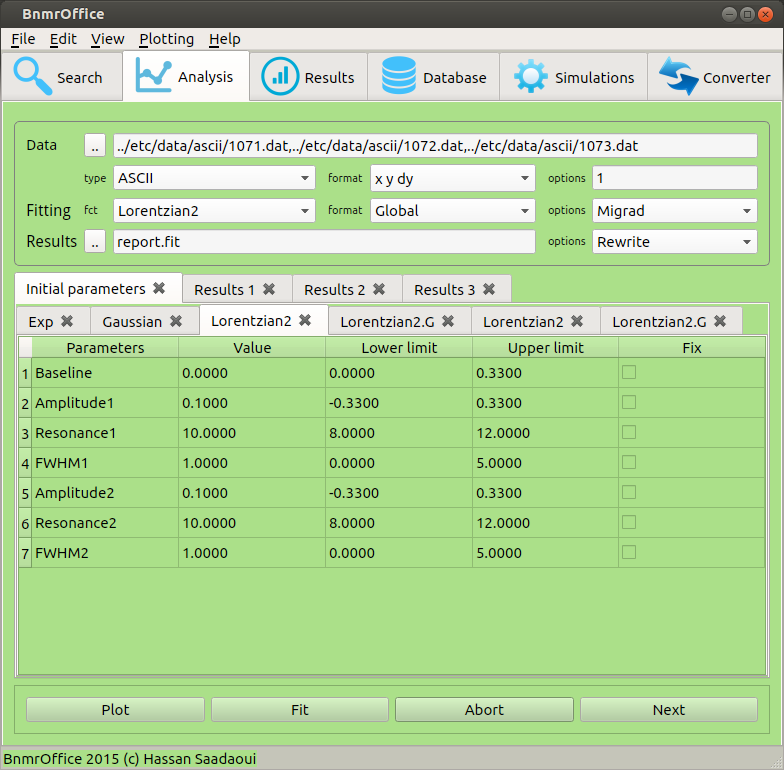
\includegraphics[width=\textwidth]{bnmroffice.png}
 \caption{Regression page of the \bof\ graphical user interface.}
 \label{fig-dep}
 \end{figure}

\section{Requirements}
The program is developed in \cpp\ and \qt. The latter provides many excellent libraries for programming and building the graphical user interface. Many desktops of Linux OS are build using \qt, such as the KDE desktop. \qt\ is cross-platform, modern and well-maintained.
The \bof's core components are as shown in Fig. \ref{fig-dep}
\begin{itemize}
 \item \qt: a \cpp\ framework for programming and developing GUI applications. Version 4.8.x or 5.x is needed.
 \item \mud: a library to read the $\mu$SR data format (.msr) developed at \cmms\ in \triumf.
 \item \minuit: a minimization routine for fitting data. 
 \item \xmgr: an application to plot and visualize data. 
 \item \qcp: to plot data directly onto the GUI (included within the package). 
 \item \gsl: (optional) for compiling few fitting functions.
\end{itemize}

In addition to the above requirements, and depending on your system, you may also need some dependency packages. The main packages are:
\begin{itemize}
 \item \texttt{gcc} compiler
 \item \texttt{automake} 
\end{itemize}

\begin{figure}[h]
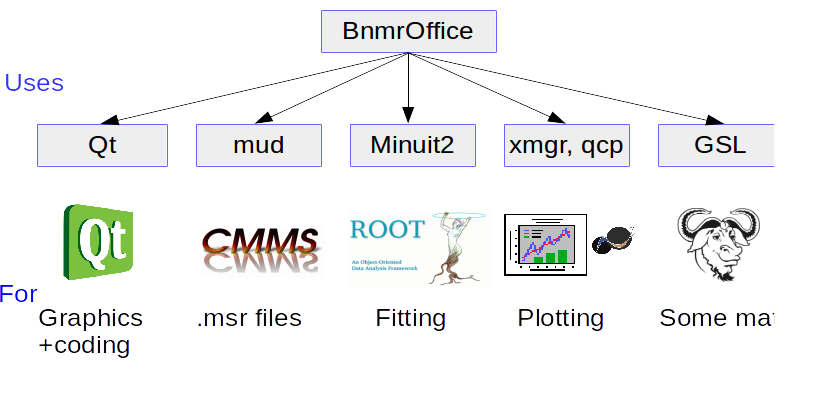
\includegraphics[width=\textwidth]{dependency.png}
 \caption{External packages required by \bof.}
 \label{fig-dep}
 \end{figure}


\newpage

\section{Package Structure}
The package you download will have a structure as shown 
in \fig{fig-str}. The main folder contains 4 sub-folders and 5 files.
\begin{itemize}
 \item \verb+src/+: contains the source code. This has also
 many sub-folders for each page and a \verb+main.cpp+, 
 \verb+mainwindow.(cpp,ui,h)+, \verb+plotting.(cpp,h)+, and
 \verb+constants.h+ for some shared constants.
 \item \verb+fct/+ contains the fitting functions and script \verb+./compile+
 to execute the codes and create the libraries.
 \item \verb+etc/+ for documentation, images, data, scripts
and templates, and the resources.qrc file needed by \qt.
\item \verb+bin/+ where the execution binary data is dumped.
 \item \verb+bnmroffice.pro+ used to generate the makefile.
 \item  \verb+AUTHOR+ for authorship attributions.
 \item \verb+LOG+ for keeping a log of the package changes over time.
 \item \verb+COPYING+ supplies the GPL agreement.
 \item \verb+README+ for installation instructions.
 \end{itemize}
\begin{figure}[h]
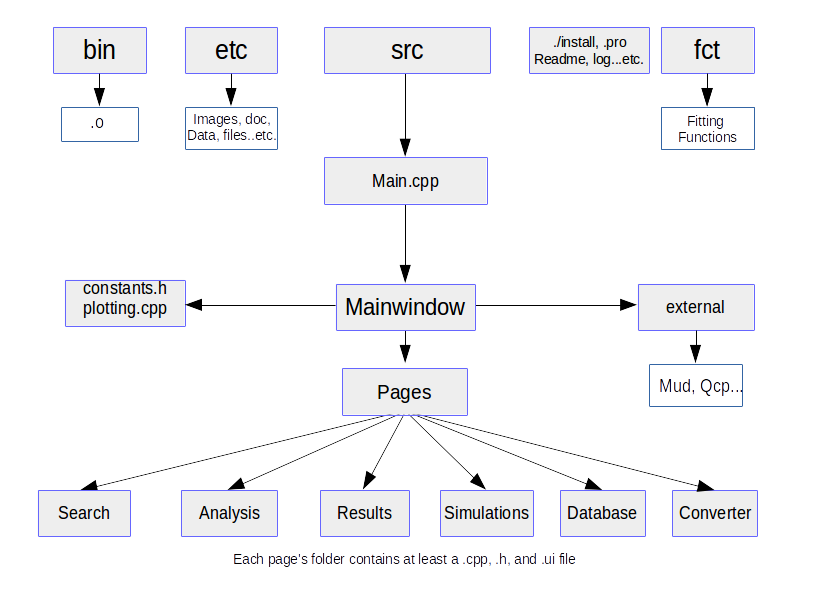
\includegraphics[width=\textwidth]{structure.png}
 \caption{Structure of the program. Upon execution,  \bof\ calls main which calls mainwindow, plotting, and constants. The mainwindow in turn calls pages and menu bar options. In each page, you find three files; .cpp, and .h for the programming part, and .ui for the GUI part.}
 \label{fig-str}
 \end{figure}
\newpage


\section{Installation}
In addition to bnmroffice, you also need: \qt, \minuit, \mud, \xmgr, and \gsl.
\begin{enumerate}
\item It is likely that your system has \qt, and \xmgr\ pre-installed. In this case, 
you only need to install \minuit\ and \mud\ libraries. 
\item These instructions may seem long, but they are meant to give as much details for the less-experienced users. In most cases, a linux-experienced user may be able to install all libraries without help, except the instructions for installing \bof.
 \item It is assumed for clarity, in all that follows, that you unpack your downloads   to the home folder \verb+~/+ (done using 
       \verb+-C ~/+ or \verb+-d ~/+). That is optional, as you may unpack somewhere else like; \verb+~/programs+, \verb+~/downloads+. 
       Without \verb+-C+ or \verb+-d+ your unpacks will appear in your current directory.
 \item  Any line here preceded by the $\$$ sign, is a command line that you may copy  and paste to your terminal. 
 \item  These instructions are meant for Linux users only. Mac users may find them useful, and Windows is not supported yet.
 \item Download the latest bnmroffice from local computers, sourceforge, or github.\\
\verb+$ wget https://sourceforge.net/projects/bnmroffice/files/bnmroffice.tar.gz/download+
 \item  Unpack it  \\     \verb+$ctar -xvf bnmroffice.tar.gz -C ~/+
\end{enumerate}


\subsection{\qt}
It is the backbone of the GUI and programming. Download the \qt\ on-line installer from \url{http://www.qt.io/download-open-source/}. It is a light executable which downloads based on your system/selections. It provides all \qt\ 5.x binary and source packages and latest \qt\ creator.


\subsection{\minuit}
This package is used for minimization. It is developed at CERN originally in Fortran and later converted to \cpp. It is very powerful
and well tested. To compile, follow these steps.
\begin{enumerate}
 \item  Download latest Minuit2 located at\\
\url{http://seal.web.cern.ch/seal/snapshot/work-packages/mathlibs/minuit/release/download.html}
 \item Unpack and cd\\
      \\     \verb+$ tar -xvf minuit.tar.gz -C ~/+
      \\     \verb+$ cd ~/minuit+

 \item  To install follow the instructions at
\\   \url{http://seal.web.cern.ch/seal/snapshot/work-packages/mathlibs/minuit/gettingStarted/autoconf.html}

 \item  Make SURE that the tests in the tutorial are running as described in the link \\ \url{http://seal.web.cern.ch/seal/snapshot/work-packages/mathlibs/minuit/gettingStarted/testOutput.html}
  \item Copy (as superuser) the miniut libraries from   
  \verb+minuit/src/.lib/liblcg_Minuit.*+ to \verb+/usr/lib/+ 
  \\ \\ \verb+$ sudo cp minuit/src/.lib/liblcg_Minuit.* /usr/lib/+

  \item Update ldconfig
 \\ \\ \verb+$ sudo ldconfig+
\end{enumerate}

{\bf Extra notes}: It is somewhat a challenge to compile Minuit2. These extra notes maybe useful.
\begin{itemize}
 \item Depending on your system, you may need to modify few codes namely  src/MnUserTransformation.cpp to add  \verb+#include <cstdio>+ or  \verb+#include <cstdio.h>+ just below  \verb+#include <algorithm>+ and re-compile.

 \item Locate where libraries and header files are, hopefully in  
 \verb+/usr/local/include/Minuit2+, and \verb+/usr/local/lib/+

 \item Add the path \verb+/usr/local/lib/+ to \verb+/etc/ld.so.conf+ as described here
 \url{http://stackoverflow.com/questions/1099981/why-cant-python-find-shared-objects-that-are-in-directories-in-sys-path}\\
 \\ \verb+$ export LD_LIBRARY_PATH=/usr/local/lib+ \\ or
 \\ \verb+$ export LD_LIBRARY_PATH=/usr/local/lib:$LD_LIBRARY_PATH+

 \item Run ldconfig
 \\ \verb+$ sudo ldconfig+
\end{itemize}


\subsection{\mud}
This package is needed to read the TRIUMF .msr files.
\begin{enumerate}
 \item  Download the MUD library source archive mud.tar.gz from \url{http://musr.ca/mud}
 \\ \verb+$ wget http://musr.ca/mud/mud.tar.gz+

 \item  Unpack and cd
 \\ \verb+$ tar -zxvf mud.tar.gz -C ~/+
 \\ \verb+$ cd ~/mud+

 \item  Run make with root access (read the install instructions withing the mud package)
 \\ \verb+$ sudo make all+

 \item  Copy the files mud.h and libmud.a into \verb+/usr/lib/+ and 
 \verb+/usr/include/+
 \\ \verb+$ sudo cp ./lib/libmud.a /usr/lib/+
 \\ \verb+$ sudo cp ./src/mud.h /usr/include/+
\end{enumerate}


\subsection{\xmgr}
This is needed for plotting. It is an old but quick and robust GUI, and makes publication quality figures. Subsequent versions have been developed, however most of the user community still prefers an outdated version dating back to 1994. Recently, a resurrected version of the outdated program appeared on Github almost 20 years later! Please contact  for other options if you are unable to install \xmgr.
\begin{enumerate}
 \item  downloand and Unpack  xmgr from https://github.com/mlund/xmgr-resurrection
 \\ \verb+$ wget https://github.com/mlund/xmgr-resurrection/archive/master.zip+
 \\ \verb+$ unzip master.zip -d ~/+
 \\ \verb+$ cd ~/xmgr-resurrection-master+

 \item  XMGR has a feature of displaying the copyright each time it starts from a terminal.
     This can obscure the user from seen the error messages produced by bnmroffice.
     To avoid this, comment the lines 107-111 in main.c and save.

 \item  Typically the following packages are required: libice-dev libx11-dev lesstif2-dev libxmu-dev libxpm-dev.
     Install if not found in your OS. Try, on ubunto/related systems, get-all (or your system's alternative).
 \\ \verb+$ sudo get-all install libice-dev libx11-dev lesstif2-dev libxmu-dev libxpm-dev+

 \item  Read README.md to compile the code. Each system is different; try these given steps:
 \\ \verb+$ cmake . -DENABLE_NETCDF=on+
 \\ \verb+$ cmake . -DCMAKE_INSTALL_PREFIX=/usr/local+
 \\ \verb+$ make+
 \\ \verb+$ sudo make install+

 \item  If all went well, open the executable \verb+xmgr+ located likely in \verb+src/+ or somewhere else within your folder.

 \item  You must locate this file and copy it to \verb+/usr/bin+ and \verb+/usr/local/bin/+ if it is not already there.
   \\  \verb+$ sudo cp xmgr /usr/bin/+
   \\  \verb+$ sudo cp xmgr /usr/local/bin/+
\end{enumerate}


\subsection{\gsl}
This package is optional. It is only needed to compile
few fitting functions in \verb+fct/+
\begin{enumerate}
 \item  download latest gsl from \url{http://gnu.mirror.iweb.com/gsl/}

 \item Unpack and cd
  \\  \verb+$ tar -xvf gsl-latest.tar.gz -C ~/+
  \\  \verb+$ cd ~/gsl-latest+

 \item  Run configure
  \\  \verb+$ ./configure+

 \item  Run make
  \\  \verb+$ make+

 \item  Run make install as root
  \\  \verb+$ sudo make install+

 \item  Update libraries cache
  \\  \verb+$ sudo ldconfig+
\end{enumerate}



\subsection{\bof}
\begin{enumerate}
 \item  cd to the downloaded package
  \\  \verb+$ cd ~/bnmroffice+

 \item  change the path to bnmr Data, and bnqr Data as defined in constants.h
  \\  \verb+$ gedit src/constants.h+

 \item  If Qt binaries are not in your path, set the env (locate where qmake is)
\\    \verb+$ PATH=/usr/Qt/5.4/gcc_64/bin:$PATH + (change \verb+"/usr/Qt/5.4/gcc_64/bin"+ as per your system)
 \\   \verb+$ export PATH+

 \item  Run qmake. [Optional: to modify the default install location use 
 \verb+$qmake PREFIX=/your.new.location/]+ 
\\   \verb+$ qmake+

 \item  Run make and make install 
 \\ \verb+$ make+
 \\ \verb+$ sudo make install+ (needs root)

 \item cd to directory \verb+fct/+ and compile all the libraries using the script compile
\\ \verb+$ cd fct+
\\   \verb+$ sudo ./compile+

 \item  To test the gui, invoke
\\  \verb+$ bnmroffice+  [or \verb+$ ./bnmroffice+ if not installed as root].
\end{enumerate}

\newpage
\newpage
\section{Description of the GUI}
The GUI has a menu bar at the very top and a tab widget below it. 
This tab widget contains 6 tabs (pages): \verb+Search+, \verb+Analysis+, \verb+Results+, \verb+Database+, \verb+Simulations+, and \verb+Converter+. Each of these contains widgets that the user may change and push buttons for issuing signals. The menu bar and the pages functionalities will be described next.
\begin{figure}
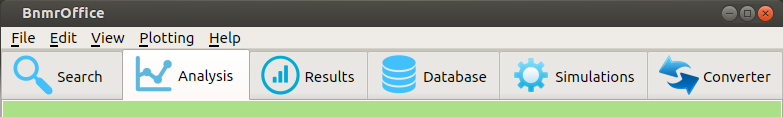
\includegraphics[width=\textwidth]{menubar.png}
 \caption{\bof\ menu bar and main pages.}
 \label{fig-menu}
 \end{figure}
\subsection{Menu bar}
\subsubsection{File}
This has 4 options; (i) invoke a new window, (ii) open an old version of \bof, (iii) clean \verb+temp.*+ data which removes all files that the program creates for plotting purposes, and (iv) quit/close the window.
\subsubsection{Edit}
It has editing options. For now, the user can overwrite the path variables of \bnmr\ and \bnqr\ archive predefined in \verb+constants.h+. Note that this is a temporary overwrite, and to make it permanent, one must modify the \verb+constants.h+ and re-compile.
\subsubsection{View}
It has the option of invoking a live/stream data window (see \ref{Streaming data}). Also, the user can change the view of the program widgets (default is \verb"fuse"), and the color of the GUI (default is \verb+"Green-white"+).
\subsubsection{Plotting}
Several check-boxes can be used for plotting purposes.
The \xmgr\ plots are closed by default after a new window is plotted to avoid the buildup of many \xmgr\ windows. To keep the old plots active one must check the box \verb+"Keep Plots"+. Also, in \xmgr, the plots are by default separated, to combine them in one plot the user could check the box \verb+"Combine Plots"+. At the moment, the GUI creates a lot of ASCII files in the background as needed by \xmgr. These files are deleted by default after the user signals are processed. If the user wants to keep copies of the ASCII file, the box \verb+"Keep ASCII files"+ must be checked.
\subsubsection{Help}
This contains the \verb+"About"+ dialog for authorship and version of the current GUI,  \verb+"Tips"+ dialog which does nothing but remind the user that by hovering the mouse index onto labels one can get the tool-tips for each widget. \verb+"Tutorial"+ invokes an HTML page with these instructions. 

\newpage
\subsection{Streaming data}\label{Streaming data}
 This window is invoked from \verb+view/show streaming window+.
 It streams data during regular intervals of time as defined by the user.
The user can choose the type of data (only \bnmrg\ is supported at the moment), run number, year, and settings for plotting options (bin, x min, x max).
The user must specify the update interval.

Upon clicking on Start, the GUI starts a counter (in seconds) and then 
plots the data after each interval. The user can change the input variables without stopping the plotting as the GUI reads the input and plots the data again at the end of the end of each interval. 

For \bnmrg\ data, at the moment, the GUI displays 4
plots and each contain 3 or 4 grouped curves. The first plot displays
the asymmetries of the experiment counters of polarized ${}^8$Li$^+$ beam. These are; the positive helicity asymmetry (defined as $\frac{counter_1 -counter_2}{counter_1+counter_2}$ during the + helicity of the laser), the negative helicity asymmetry, and the total asymmetry which is the difference of the first two. In the 2nd plot, similar asymmetries for the neutral beam are presented. In the 3rd plot, the counters of polarized ${}^8$Li$^+$ are shown, and the counts of beam monitors are shown in plot 4. An example is shown in \fig{fig-stream}

\begin{figure}[h]
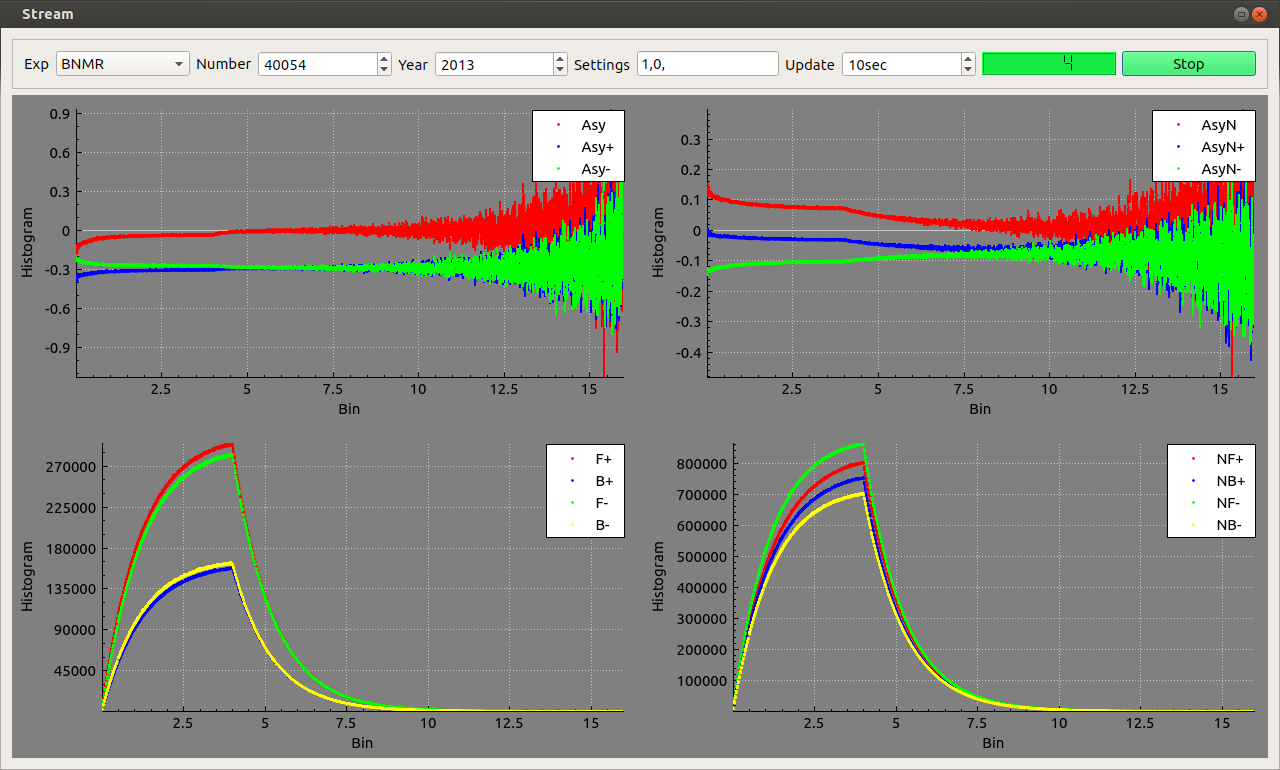
\includegraphics[width=\textwidth]{stream.png}
 \caption{Streaming window: it streams data at regular intervals. This could be useful for on-line experiments. }
 \label{fig-stream}
 \end{figure}
\newpage
\subsection{Search}
In this page, the user can find the data that corresponds to his search query. There are 9 fields that user can change. In the first line one finds, the title field (must be a string), experiment type (either \bnmr\ or \bnqr\ data at the moment), type of data (1f, 1n, 20, and 2e modes of \bnmrg\ data). In the 2nd line, the user can specify 
the intervals of year, run number and elapsed time. In the 3rd line, 
the user can specify the interval of independent variables of temperature, energy, and field. These are defined in \verb+tab_search.cpp+ code.
The user can start the search by clicking on the pushbutton \verb+Search+.
After sometime, the search results will be returned in a table with 9 columns. These are (1) check-box columns to choose which runs to send to the analysis page, (2) run number, (3) year, (4) type of experiment mode, (5) elapsed time in minutes, (6) temperature in K, (7) energy in keV, (8) field in Gauss, and (9) the run title. 

The user can also display more columns by clicking on the pushbutton \verb+"More"+ which displays a dialog that contains more fields to display. These fields are pre-defined in a template file called \verb+bnmr-bnqr-logs.txt+ which contains 5 columns, (i) Labels, (ii) Symbols, (iii) Exp, (iv) Path, and (v) Unit. The user can change this file to add more fields or to update the previous ones. The program will read the file saved in the current working directory, and if not found, it reads the default file from \verb+resources.qrc+.

The user can select all runs by clicking on \verb+"Select"+ and send the selected runs to the next page for analysis by pushing the button \verb+"Next"+.
\begin{figure}[h]
\center
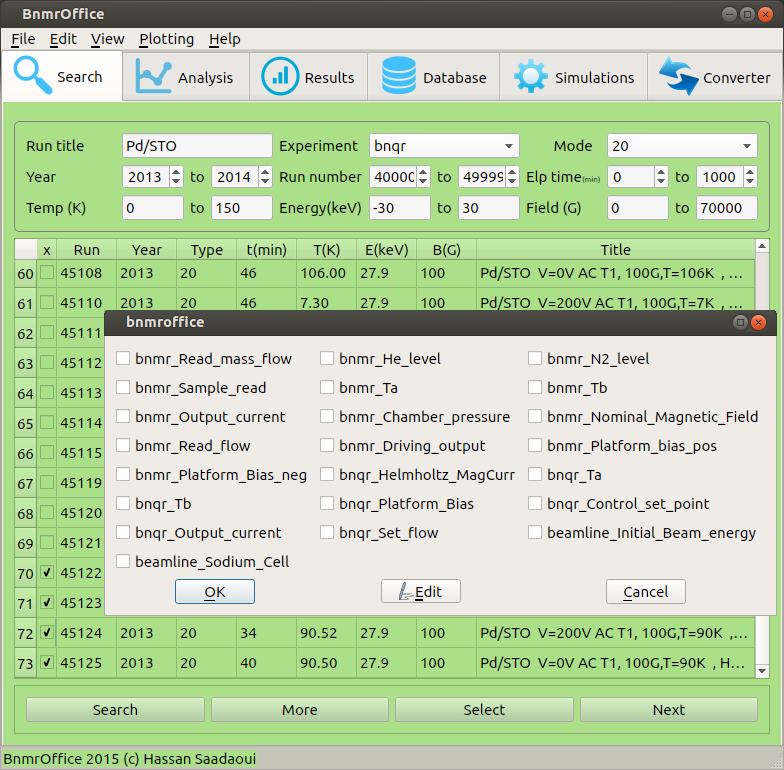
\includegraphics[width=0.8\textwidth]{search.png}
 \caption{Searching the .msr files. More fields can be displayed after clicking on "More" and checking the desired fields. These fields are predefined in \texttt{"bnmr-bnqr-logs.txt"} which can be edited by pushing \texttt{"Edit"}.}
 \label{fig-mag}
 \end{figure}

\clearpage
\subsection{Regression}
This is the main page of the entire program and by far the most complicated to program. The network of background signals are large and may cause the program to crash unexpectedly. Please report these cases.  
% \begin{figure}[h]
% 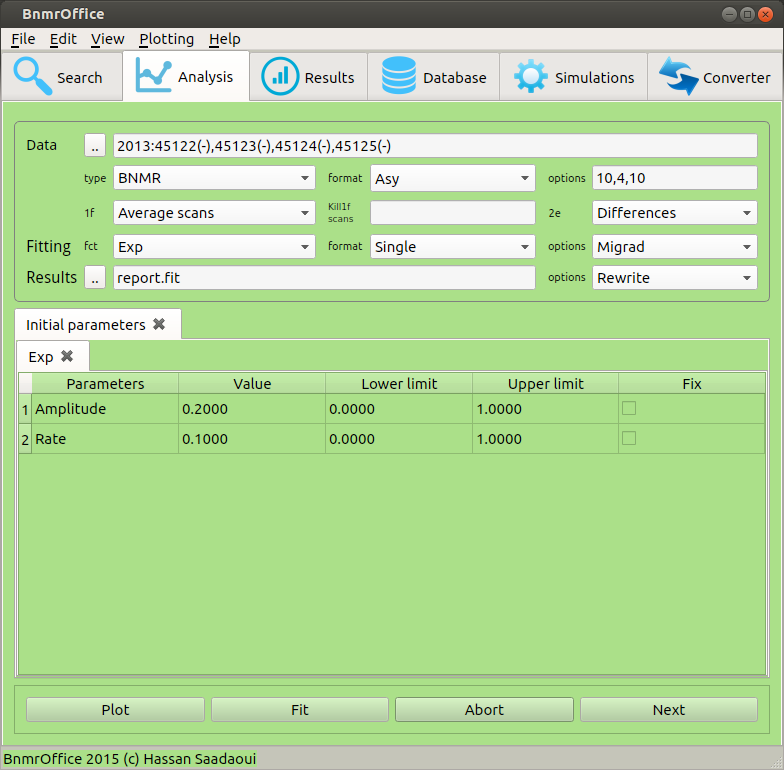
\includegraphics[width=\textwidth]{analyze1}
%  \caption{Regression analysis page}
%  \label{fig-mag}
%  \end{figure}

\subsubsection{Data input}
\begin{figure}[h]
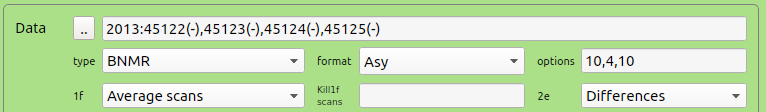
\includegraphics[width=\textwidth]{analyze-bnmr.png}
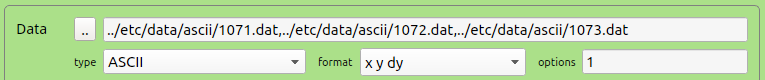
\includegraphics[width=\textwidth]{analyze-ascii.png}
 \caption{Options for data input}
 \label{fig-mag}
 \end{figure}
The user can choose to fit either ASCII text data or \verb+.msr+ files of the \cmms\ facility. The user can locate the data using the tool button next to Data for ASCII files. For \verb+.msr+ files, the user can only specify the run year and number and the program looks it up in the archive directory (defined in \verb+constants.h+ or \verb+Edit+).
For each of these types of data, there are three ways to specify the input data.  For the \verb+.msr+ type follow these instructions;

\begin{enumerate}
\item Using run numbers directly:
\begin{itemize}
\item  A year must always be specified.
\item  "|" is used to separate runs of different years.
\item  "," (coma) separates between run numbers.
\item  "-" separates between two numbers, which defines a range of runs.
\item  "(-)" is used to flip the asymmtry opposite to the original one, (either up or down). 
\item  No other characters or space are allowed. 
\item Example 1: "2011:45012,45672,42333|2013:45333(-),40123"
\item Example 2: "2011:40100-40110"
\end{itemize}
\item Using \verb+.inf+ files:
\begin{itemize}
\item It is best to create \verb+.inf+ file out of \verb+temp.inf+ created by the program from a direct input method above.
\item The file \verb+temp.inf+ is found in the working directory.
\item Must follow the same template as of \verb+temp.inf+
\item The user can change the file and update the independent variables.
\end{itemize}
\item Using \verb+.list+ files 
\begin{itemize}
\item The content of the file must follow the same instructions as run numbers.
\item Example: A file named \verb+"myfavoriteruns.list"+, contains a single line\\ \verb+2010:45012,45672,41223,45012,40072,42313|2014:45123(-),40003+.

\end{itemize}
\end{enumerate}

 Reading/fitting ASCII files follows very similar instruction to above. 
Files to fit should be either written in the lineEdit (separated by commas) or; in files of \verb+.list+ or \verb+.inf+ extension as above. The file must reside in the working directory, otherwise its full name with path should be given. Examples;
\begin{itemize}
\item Direct input: "file1.txt,file2.txt,file3.txt"
\item \verb+.list+ file: contains a single ascii line:\\ \verb+"file1.txt,file2.txt,file3.txt"+
\item \verb+.inf+ file: \verb+"myruns.inf"+, contains the columns\\
files year temp\\
file1.txt 2015 100\\
file2.txt 2014 200\\
file3.txt 2015 300\\
\end{itemize}

The format of  \verb+.msr+ files to create are pre-defined as asymmetry or counts and are all in xydy format. The inner format of the ASCII file must be set in the field \verb+format+ and these must be columns with numbers and no other characters. 

For the \verb+.msr+ files, there are several more options to tweak, such as the averaging of 1f runs, ignoring some bad 1f scans, and setting the type of 2e asymmetry. An experienced \bnmrg\ user must be familiar with these options. 

The data can be binned and the limits of xmin and xmax values can be set in the options (settings) field. These must be numbers separated by commas.




\subsubsection{Fitting selection}
\begin{figure}[h]

\includegraphics[width=\textwidth]{analyze-fct.png}
 \caption{Fitting functions input.}
 \label{fig-mag}
 \end{figure}

The user can select the function to use, the mode of fitting (single or global) and type of errors. The functions are defined in the folder \verb+fct/+ and the user can add new ones by invoking the selection \verb+"Create New"+ in the functions comboBox. The user must follow the instructions in the pop-up window and then select \verb+"Update"+ from the comboBox. This will add the newly defined function to the list. 

For the global method the user can choose to show all parameters for each run or not. These settings can be changed by double clicking on the initial parameters tab-widget. 

The errors are defined by \minuit\ routine, and are symmetric (Migrad) or asymmetric (Minos) errors. The latter are heavy to compute and the program may become unresponsive for sometime while the computation is going on. For further details read \url{http://seal.web.cern.ch/seal/documents/minuit/mnerror.pdf}.
\subsubsection{Results output}
\begin{figure}[h]

\includegraphics[width=\textwidth]{analyze-res.png}
 \caption{Fitting results output.}
 \label{fig-mag}
 \end{figure}
The fitting results are written to this file. The user must specify a name, or browse for an old file. The results can be either appended
 (using \verb+Append+) to the old file keeping its content (useful for doing run by run fitting), or the old file is overwritten using \verb+Rewrite+. 
\subsubsection{Parameters input}\begin{figure}[h]
\center
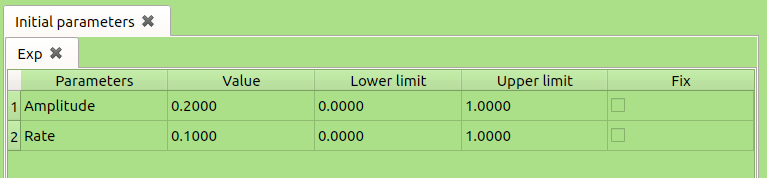
\includegraphics[width=.75\textwidth]{analyze-table-s.png}
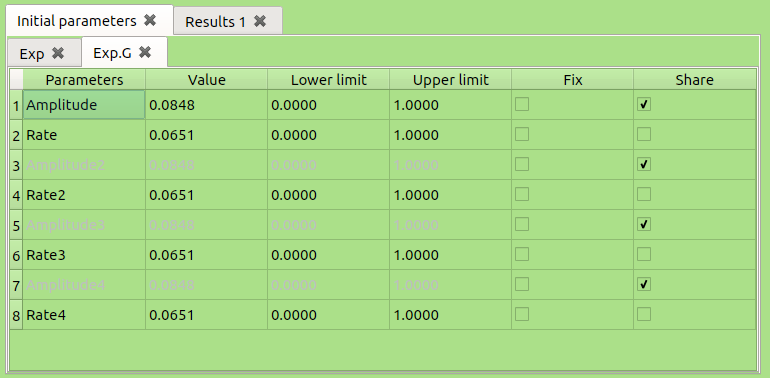
\includegraphics[width=.75\textwidth]{analyze-table-g.png}
 \caption{Input parameters for (a) single and (b) global fits. (a) The fit starts from this table for each file, or from the results of the last file in the sequence enabled by double clicking on the \texttt{"initial parameters"}. (b) If a parameter is shared between files, only the parameter of the first run is active and the same parameter for other files becomes inactive. }
 \label{fig-tables}
 \end{figure}
The initial parameters are read from the function library.
The table contains 5 columns for the single method, and 6 columns for the global method. These columns are; (1) parameter name, (2) initial value of the parameter, (3) lower limit, (4) upper limit, (5) fix the parameter checkBox, and (6) share the parameter checkBox.

These parameters can be changed, and saved in a template for future use  by right-clicking on the specific table and then choose \verb+"save as a template"+. This creates a text file template with a prefix \verb+".tab"+. The  user can change this text file as required, and the template can be loaded later for a similar function.
\subsubsection{Parameters output}
\begin{figure}[h]
\center
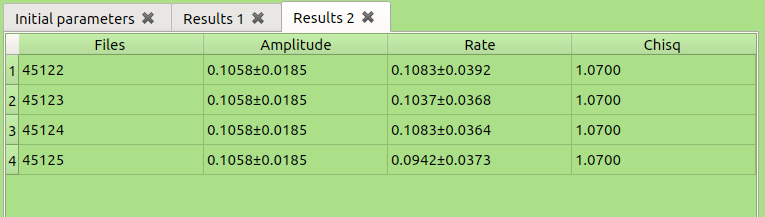
\includegraphics[width=.75\textwidth]{analyze-res-g.png}
 \caption{Results of a global fit where the shared parameter is Amplitude. }
 \label{fig-tables}
 \end{figure}
This prints out the output of the fit. The number of significant figures can be set by double-clicking on the results tab. One can also change the number of errors to show, and the way the filename is displayed.


\clearpage
\subsection{Results}
This page reads the files of fitting parameters created by the
analysis page. It displayed a table with two columns, the left column represents the x-axis and the right column the y-axis.
Each column contains all fields found in the specified file (as created during the fitting). 

The user can check any of the fields, and a matrix of plots of y versus x will be displayed.  The user can clear all choices using \verb+"Clear"+, and kill/delete the active table using \verb+"Purge"+. 

The plots are made using \xmgr\ plotting program. Horizontal or vertical error bars are displayed if specified in the chosen parameter. The user can edit the \xmgr\ windows as he pleases and can make publication quality figures out of these results.
\begin{figure}[h]
\center
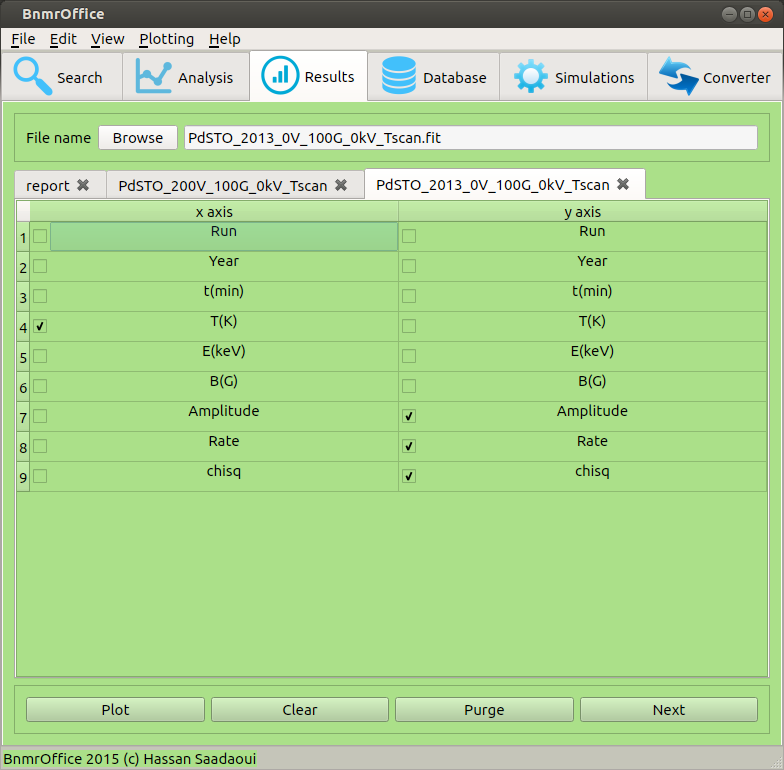
\includegraphics[width=\textwidth]{results1.png}
 \caption{Results page.}
 \label{fig-results}
 \end{figure}


\newpage
\subsection{Database}
This page offers a user-friendly interface for databases, and
uses SQLite language \url{http://www.tutorialspoint.com/sqlite/sqlite_overview.htm}. At the start, the user must select a database by clicking on the toolButton next to \verb+"Database"+, or create a new one from the \verb+"Querry"+ lineEdit using SQL commands and hitting \verb+"Execute"+.
It is advised to use an SQL manager (like the friendly browser extension SQLite manager) to create databases and tables. Then, one can use this interface to add/delete rows and edit cells, interact with the content of the database. But an experienced user can do everything from this page as well by executing the \verb+"Querry"+ commands.


Te get familiar with the interface two databases are pre-made and come with the program and can be found in the folder \verb+"etc/sql/"+. These are called \verb+"bnmr.sqlite"+ and \verb+"physics.sqlite"+. Each contain several tables. The user can load any of these tables from the comboBox, and a model of the table will be displayed. 

The user can execute any query to study the loaded table. Example;\\ \verb+SELECT * FROM table_of_constants where Unit="kg"+ will select all fields in the \verb+table_of_constants+ where the unit is in kg. The user must be familiar with SQL to execute from the Query field. Any table can be changed by adding or deleting rows. Also each cell can be edited, or displayed by clicking on \verb+"Open"+. This can be used to display a cell with a lot of text or view the cell as image if the full path of the image was given in that cell. 
\begin{figure}[h]
\center
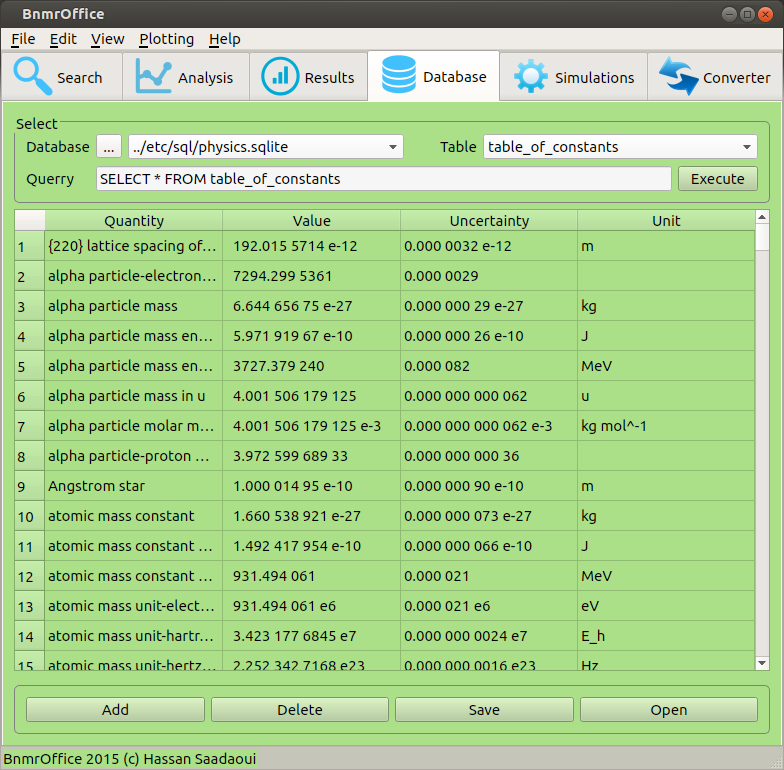
\includegraphics[width=0.8\textwidth]{database1.png}
 \caption{Database interface loaded with a table of physical constants.}
 \label{fig-mag}
 \end{figure}

 \clearpage
\subsection{Simulations}
\subsubsection{Van-Vleck second moment}
In this page, one computes the dipolar second moment using the Van-Vleck method [J. H. Van Vleck, Phys. Rev. 74, 1168 (1948)]. The user specifies the implanted ions, target material, and type of lattice, and then the coordinates of each site. The results will be plotted on the same page using \qcp\ libraries. The plots can be exported into .pdf, .png, and .bmp files. ASCII files of the computed are created in the working directory.

The simulation is tested against two published papers in (1) Lattice locations of 8Li in Cu, Hyperfine Interactions 120/121 (1999) 419-422. (2) Location of 12B in Al and Cu, Phys Rev B 13, 34 (1976). The source code of this calculation is originally written by Samir Tabara, and adapted for \bof.
\begin{figure}[h]
\center
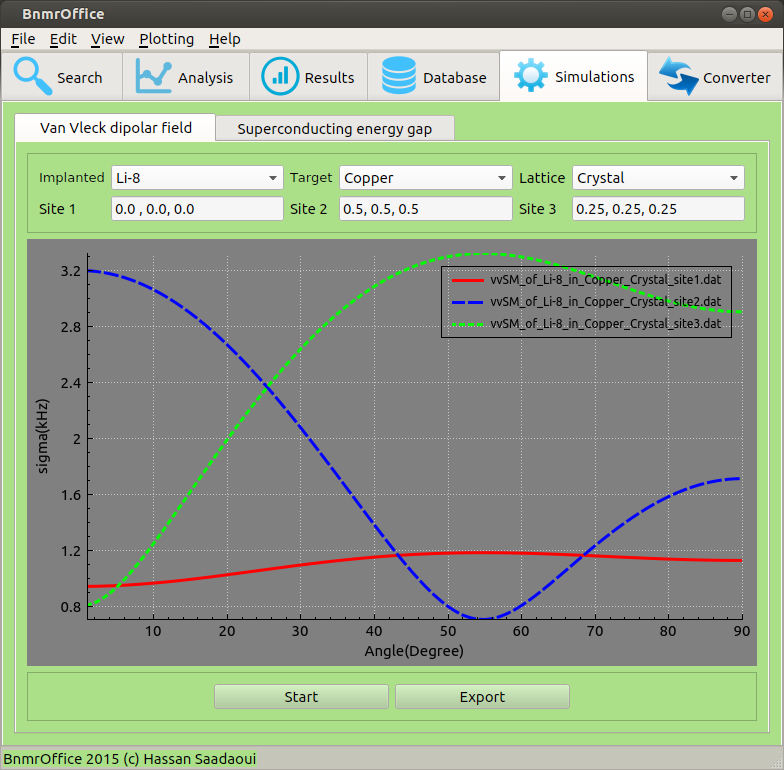
\includegraphics[width=\textwidth]{sim-vv.png}
 \caption{Van-Vleck calculation}
 \label{fig-mag}
 \end{figure}

 \clearpage

\subsubsection{Superconducting energy gap}
This page performs calculation of the superconducting energy gap, for a given gap symmetry and parameters such as the penetration depth and coherence length. The definitions can be found in the papers 
H. Saadaoui \etal, Phys. Rev. B 88, 094518 (2013), and
R. Prozorov and R. W. Giannetta, Supercond. Sci. Technol. 19, 41 (2006). 

The simulation computes three functions, the second moment of the magnetic field distribution versus temperature (\verb+sigma_vs_temp+), the second moment of the magnetic field distribution versus field (\verb+sigma_vs_field+), and the penetration depth versus temperature (\verb+lambda_vs_temp+).

Four forms of the energy gap $\Delta(T,{\bf k})$ are pre-defined; the $s$-wave, $d$-wave, $s$-wave-dirty and $d$-wave non-monotonic.  These are defined in Eqs. 17 and 18 in the Prozorov paper. Two empirical forms of the second moment of the magnetic field distribution versus field are specified, the Modified-London and Ginsburg-Landau forms. Please refer to the paper of H. Saadaoui \etal, Phys. Rev. B 88, 094518 (2013) for further details about these functions.

\begin{figure}[h]
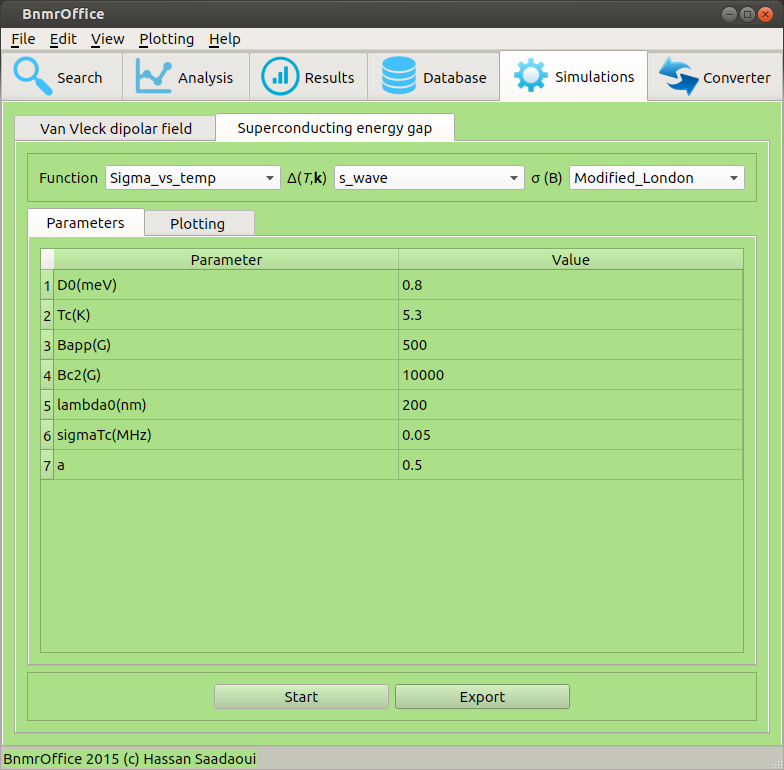
\includegraphics[width=0.5\textwidth]{sim-eg-in.png}
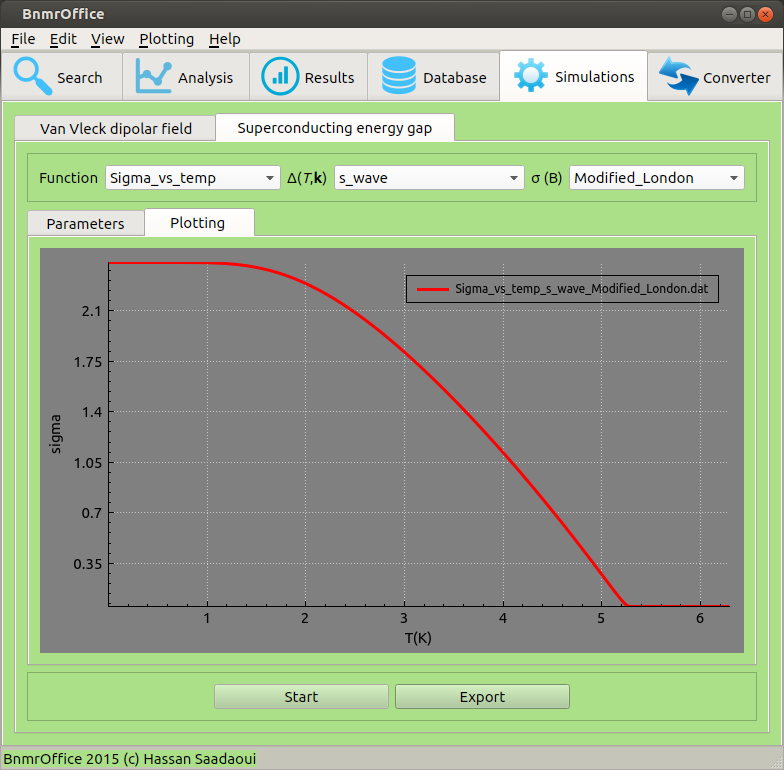
\includegraphics[width=0.5\textwidth]{sim-eg-out.png}
 \caption{Input and output of the energy-gap interface}
 \label{fig-mag}
 \end{figure}

 \clearpage
\subsection{Converter}
This page is used to convert between several units useful for a \bnmrg\
user. The definitions are given in \verb+"tab_convert.cpp"+ file. The user can change any field and hit Enter, and the associated field will update.
\begin{itemize}
\item Magnetic Field (G)  = Frequency (kHz)/0.63015
\item Magnetic Field (G)  = 2.2131*Current(Amp) + 0.175
\item Pulse duration (ms) =  5*10000/$\pi$/Bandwidth(Hz)
\item Pulse duration (ms) =  1764.8/Bandwidth(Hz)
\item Magnetic Field (G) =  Frequency (kHz)/85.16
\end{itemize}
\begin{figure}[h]
\center
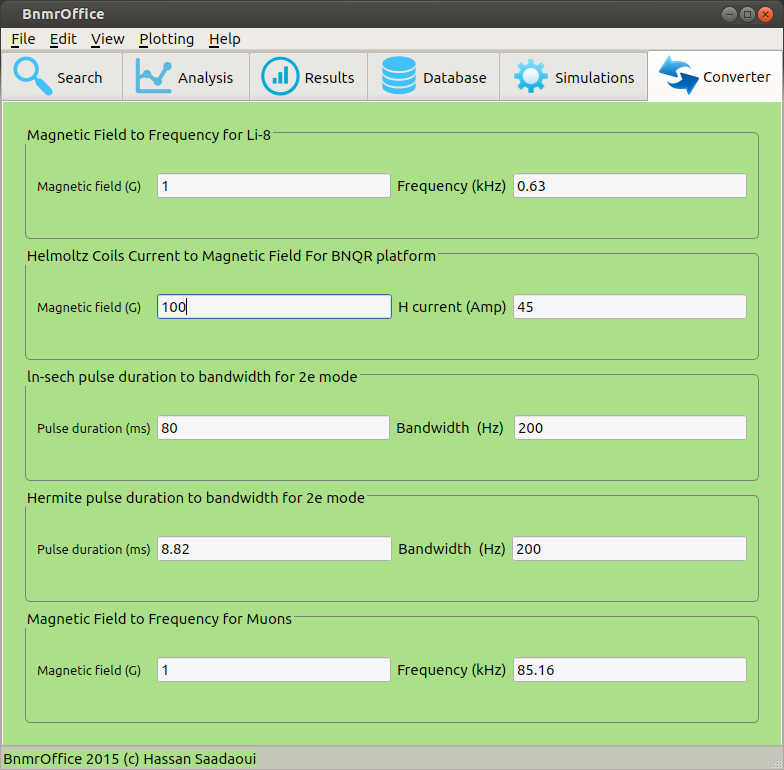
\includegraphics[width=\textwidth]{converter.png}
 \caption{Converter page.}
 \label{fig-mag}
 \end{figure}

\section{Fitting functions}
The user can write his own fitting functions in the directory \verb+fct/+.
A new function must be written in \cpp\ but requires minimal programming knowledge of this language. 
At template of a typical function is as follows:
%\begin{verbatim}
\begin{lstlisting}[language=C++, keywordstyle=\color{red}]
#include <iostream>
#include <fstream> 
#include <math.h>
#include <stdio.h>
#include <vector>
#include <sstream>   
#include <string.h>
#include <iostream>
using namespace std;
#include "parameters.h"

//Wrap in "C" for the compiler.
extern "C" 
{ 
  //The defalt initial parameters loaded to the table.
  void defaultParameters(Parameters &defaults)
  {
    defaults.addParameter( "Amplitude" , 0.2, 0.001, 0.15, 1.0 );//par[0]
    defaults.addParameter( "Rate"      , 0.1, 0.001, 0.0,  1.0 );//par[1]
  }
  //This must have the same number of parameters as in the default parameters above.
  double function(double x, const std::vector<double> par)
  {
  	return par[0]*exp( - par[1]*x);//par[0] is amplitude and par[1] is rate.
  }
}
\end{lstlisting}
%\end{verbatim}
The user must follow these instructions:
\begin{itemize}
\item Make a copy of the file \verb+newFunction.cpp+ found in \verb+etc/files+.
\item Rename the file (eg: newfct.cpp) and save it in the folder \verb+fct/+.
\item cd to the directory fct, and run the script \verb+./compile+ as root
\item \texttt{$\$$ sudo ./compile name}   (eg: sudo ./compile newfct.cpp)
\item This compiles the library and puts a copy in the library functions folder (\verb+/opt/bnmroffice/lib/+).
\end{itemize}
% \section{Modifying the program}

\end{document}
